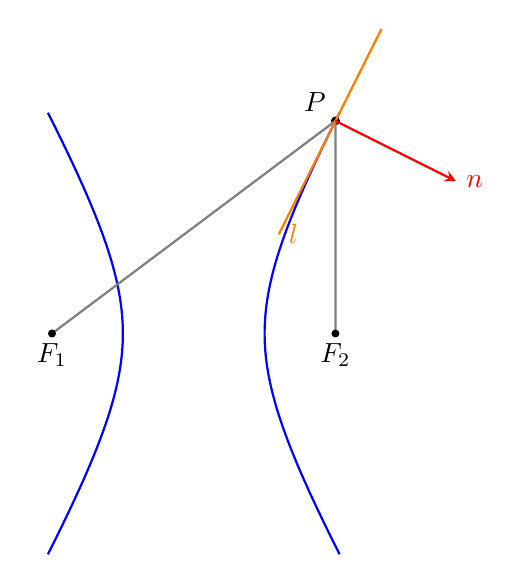
\begin{tikzpicture}[scale=.9,>=stealth]
\draw[blue,thick,domain=-1.35:1.35,samples=90] plot ({cosh(\x)},{sqrt(3)*sinh(\x)});\draw[blue,thick,domain=-1.35:1.35,samples=90] plot ({-cosh(\x)},{sqrt(3)*sinh(\x)});
\coordinate (P) at (2,3);\fill (P) circle (1.8pt) node[above left] {$P$};
\draw[gray,thick] (P)--(-2,0);\fill (-2,0) circle (1.6pt) node[below] {$F_1$};
\draw[gray,thick] (P)--(2,0);\fill (2,0) circle (1.6pt) node[below] {$F_2$};
\draw[orange,thick] (2.65,4.3)--(1.2,1.4) node[right] {$l$};
\draw[->,red,thick] (P)--(3.7,2.15) node[right] {$n$};
\end{tikzpicture}
